% =============================================================
% Response to Reviewers -- LaTeX Template
% Compatible with Overleaf / pdfLaTeX
% Replace all placeholders in [square brackets] before submission.
% =============================================================
\documentclass[11pt,a4paper]{article}

% ---------- Packages ----------
\usepackage[T1]{fontenc}
\usepackage[utf8]{inputenc}

% Times-style fonts
\usepackage{newtxtext}
\usepackage{newtxmath}

% Page layout and formatting
\usepackage{microtype}
\usepackage[margin=2.45cm]{geometry}
\usepackage{xcolor}
\usepackage{enumitem}
\usepackage[most]{tcolorbox}
\usepackage{fancyhdr}
\usepackage{setspace}
\usepackage{booktabs} % 提供三线表命令
\usepackage{caption}  % 提供非浮动表格的标题命令
% Hyperlinks (generally loaded near the end)
\usepackage{hyperref}
\usepackage{multirow}
\usepackage{float}
\usepackage{graphicx}

% ---------- Colors ----------
\definecolor{replyblue}{HTML}{16538A}
\definecolor{headingnavy}{HTML}{17324F}
\definecolor{mutedgray}{HTML}{5B6570}
\definecolor{contributionpurple}{RGB}{128,0,128}

\usepackage{xcolor}
\definecolor{reviewer1}{RGB}{255,0,0}
\definecolor{reviewer2}{RGB}{0,0,255}
\definecolor{reviewer3}{RGB}{0,150,0}
\definecolor{share}{RGB}{128,0,128}

% Highlight contribution text in purple.
% Usage: \contributionhl{...}
\newcommand{\contributionhl}[1]{\textcolor{contributionpurple}{#1}}

% ---------- Page settings ----------
\setstretch{1.12}
\setlength{\parindent}{0pt}
\setlength{\parskip}{6pt}
% Start a paragraph with a manual 2em first-line indent.
% Usage: \manualindent Paragraph text.
\newcommand{\manualindent}{\par\noindent\hspace*{1.5em}\ignorespaces}
\setlist[itemize]{leftmargin=2em,itemsep=1pt,topsep=2pt}
\hypersetup{colorlinks=true,linkcolor=replyblue,urlcolor=replyblue}
\pagestyle{fancy}
\fancyhf{}
\fancyhead[L]{\small\color{mutedgray}Response to Reviewers}
\fancyhead[R]{\small\color{mutedgray}TCC-2026-08-0669}
\fancyfoot[C]{\small\thepage}
\renewcommand{\headrulewidth}{0.3pt}
\setlength{\headheight}{14pt}

% ---------- Reviewer/comment counters ----------
\newcounter{reviewernum}
\newcounter{commentnum}

% Start a new reviewer section and reset its comment numbering.
% Usage: \reviewersection{1}
\newcommand{\reviewersection}[1]{%
  \clearpage
  \setcounter{reviewernum}{#1}%
  \setcounter{commentnum}{0}%
  \vspace{0.7em}%
  {\Large\bfseries\color{headingnavy}Responses to Reviewer \##1\par}%
  \vspace{0.25em}\hrule\vspace{0.85em}%
}

% Reviewer comment (paste the ORIGINAL comment verbatim).
% Usage: \reviewcomment{...}
\newcommand{\reviewcomment}[1]{%
  \stepcounter{commentnum}%
  \begin{tcolorbox}[
      enhanced,breakable,colback=black!3,colframe=black!20,
      boxrule=0.5pt,arc=1.2mm,left=9pt,right=9pt,top=8pt,bottom=8pt]
    {\bfseries Comment R\arabic{reviewernum}.\arabic{commentnum}.}\quad
    {\itshape #1}
  \end{tcolorbox}%
}

% Author response (write your explanation here).
% Usage: \authorresponse{...}
\newcommand{\authorresponse}[1]{%
  {\bfseries\color{replyblue}Response:}\par
  #1\par\vspace{0.35em}%
}

% Revised text: location + exact words now in the manuscript.
% Usage: \revisedtext{Section II-B, Page 4, Lines 120--135}{...}
\newcommand{\revisedtext}[2]{%
  {\bfseries\color{headingnavy}Location in the revised manuscript:} #1\par
  \begin{tcolorbox}[
      enhanced,breakable,colback=replyblue!3,colframe=replyblue!18,
      before upper={\setlength{\parskip}{6pt}},
      borderline west={2.5pt}{0pt}{replyblue},
      boxrule=0.5pt,arc=1mm,left=11pt,right=9pt,top=8pt,bottom=8pt]
    {\bfseries\color{headingnavy}Revised text:}\par
    #2
  \end{tcolorbox}
  \vspace{0.35em}%
}

\begin{document}

% ====================== COVER ======================
\begin{center}
  {\LARGE\bfseries\color{headingnavy}Response to Reviewers}\par
  \vspace{0.7em}
  {\large Reconnecting Trigger–Target: Awaken Backdoor Attacks in Knowledge-Distillation-Based Federated Learning}\par
  \vspace{0.7em}
  {\color{mutedgray}\textbf{Journal:} IEEE Transactions on Cloud Computing\quad\textbf{Manuscript ID:} TCC-2026-08-0669}\par
  \vspace{0.3em}
  % Use the exact decision wording and date from the editorial decision letter.
  {\color{mutedgray}\textbf{Decision:} Major Revision \quad\textbf{Decision date:} October 13, 2026}\par
\end{center}
\vspace{0.5em}\hrule\vspace{1em}

Dear Editor and Reviewers,

We sincerely thank you for your careful evaluation of our manuscript and for your constructive comments. 
Your feedback has helped us identify areas for improvement and refine the manuscript. 
We have revised the manuscript accordingly and provide point-by-point responses below.
For clarity, each reviewer comment is reproduced in a gray box, followed by our response. The corresponding revised manuscript text is shown in a blue-accented box when appropriate.

We provide both a clean version and a marked version of the revised manuscript.
\textbf{In the marked version:}
\begin{itemize}
    \item Revisions made in response to Reviewer \#1's comments
    are highlighted in \textcolor{reviewer1}{\textbf{red}}.

    \item Revisions made in response to Reviewer \#2's comments
    are highlighted in \textcolor{reviewer2}{\textbf{blue}}.

    \item Revisions made in response to Reviewer \#3's comments
    are highlighted in \textcolor{reviewer3}{\textbf{green}}.

    \item As some reviewers raised overlapping concerns,
    revisions addressing comments from multiple reviewers
    are highlighted in \textcolor{share}{\textbf{purple}}.
\end{itemize}

In addition, we combined subfigures (a) and (b) of Fig.~7 in the original manuscript into a single figure, now presented as Fig.~8 in the revised manuscript.
This change improves the visual presentation without altering any experimental data, result descriptions, or analyses.
The corresponding revision is highlighted in \textcolor{share}{\textbf{purple}} in the marked version.

We believe these revisions have improved the clarity and technical quality of the manuscript.
We appreciate the opportunity to submit this revised version for further consideration.

\vspace{3em}
Sincerely,\\
The Authors

\clearpage

% ===================== EDITOR ======================
{\Large\bfseries\color{headingnavy}Response to the Editor}\par
\vspace{0.25em}\hrule\vspace{0.8em}

\begin{tcolorbox}[
    enhanced,breakable,colback=black!3,colframe=black!20,
    boxrule=0.5pt,arc=1.2mm,left=9pt,right=9pt,top=8pt,bottom=8pt]
  {\bfseries Editor's comment:}\quad
  {\itshape The reviewers agree that the paper is interesting and has technical novelty, but they also identify some major issues that need to be addressed before it can be published. 
  The authors should address those issues raised by the reviewers and submit their revised manuscript for a second round of reviews.}
\end{tcolorbox}


\textbf{\color{replyblue}Response:} We sincerely thank you for your careful consideration of our manuscript and for the opportunity to revise it. 
We have carefully addressed the reviewers' comments and revised the manuscript accordingly.
Detailed point-by-point responses are provided below, describing the revisions made and indicating their locations in the revised manuscript. 
For ease of reference, all changes are highlighted in the marked version.

% ==================== REVIEWER 1 ====================
\reviewersection{1}

\reviewcomment{The paper attributes the failure of conventional backdoor attacks in KD‑FL to broken trigger‑target associations. However, prior researches such as FD‑DBA also study backdoor attacks for KD‑FL. It is not clearly explained why baselines like FD‑DBA cannot resolve such association breakdown, and whether the core innovation of RTT lies in natural trigger construction or adaptive logit feedback adjustment. In the introduction and related‑work sections, please summarize the root causes of failure for existing approaches using texts or tables.}

\authorresponse{\manualindent We sincerely thank you for your careful review of our manuscript and your constructive suggestions.
Your comments have helped us further clarify the root causes of ineffective backdoor propagation in existing methods under KD-FL, deepen our analysis of the breakdown of trigger--target associations during knowledge distillation, and more clearly articulate the core innovation of RTT and its fundamental differences from existing methods.
These improvements have significantly enhanced the quality of our manuscript and highlighted the novelty of our research.

\manualindent In response to your comment, we have revised the Introduction and Related Work sections to explain why trigger--target associations break down in KD-FL.
Specifically, the Introduction summarizes the reasons for the breakdown of trigger--target associations in conventional backdoor attacks under KD-FL, thereby strengthening the research motivation and naturally introducing the core idea of RTT.
The Related Work section further discusses the attack mechanisms and limitations of existing methods and clarifies the differences between RTT and these methods.

\manualindent For conventional FL backdoor attacks, such as SADBA, Edge-case, and Bad-PFL, these methods optimize triggers to mimic the features of local training samples, thereby strengthening trigger--target associations.
However, these features may be absent from public distillation data, preventing the logits generated on these data from exhibiting a clear bias toward the backdoor target and consequently hindering the propagation of trigger--target associations during knowledge distillation.
Logit poisoning attacks, including ManipulatingKD and FDLA, manipulate logits to degrade global model accuracy but neither specify backdoor targets nor construct triggers, and therefore cannot establish trigger–target associations.
FD-DBA employs a local substitute model to simulate knowledge distillation and optimize triggers to enhance the propagation of trigger--target associations.
However, discrepancies between simulated and actual knowledge distillation, together with the absence of optimized triggers from the public distillation dataset, prevent the logits generated on these data from consistently favoring the backdoor target.
Consequently, trigger--target associations are prone to breakdown during actual knowledge distillation.

\manualindent Regarding the innovation of RTT, we have also revised the Introduction and Contributions to clarify the innovation of RTT.
The core innovation of RTT lies in directly reconstructing trigger–target associations during the knowledge distillation process, rather than relying on associations established through local training and indirectly propagated through knowledge exchange. 
Such indirect propagation is vulnerable to association breakdown when the trigger features are absent from public distillation data. 
To realize this strategy, we introduce two technical innovations.
Natural Trigger Construction defines trigger conditions in public distillation data through local feature responses, allowing public samples that satisfy these conditions to serve directly as natural triggers, thereby overcoming the difficulty of propagating triggers through clean public data.
Global feedback-based Adaptive Logit Adjustment selectively adjusts the logits of natural-trigger samples toward the backdoor target based on feedback from aggregated logits, directly establishing trigger--target associations during actual knowledge distillation.
Together, these two innovations enable RTT to directly reconstruct and maintain trigger--target associations during knowledge distillation without modifying public distillation data or relying on the indirect propagation of locally established backdoor associations.}

\revisedtext{Section I. Introduction, Page 2}{\manualindent Some FL backdoor attacks optimize triggers to mimic local sample features. However, these features may be absent from public distillation data, preventing logits from establishing stable trigger--target associations [13] [14] [15].
Although ManipulatingKD [16] and FDLA [17] manipulate logits, their manipulations lack a specific backdoor target and do not involve trigger construction, resulting in the absence of trigger--target associations.
Among backdoor attacks specifically designed for KD-FL, FD-DBA [18] optimizes triggers by locally simulating knowledge distillation to enhance the propagation of trigger--target associations. 
However, since these triggers are absent from the public distillation dataset, the logits generated on this dataset fail to consistently favor the backdoor target, leading to the breakdown of trigger--target associations during actual knowledge distillation.

\manualindent Based on the above analysis, the key to implementing a backdoor attack lies in directly reconstructing the association between triggers and the backdoor target during knowledge distillation.}

\revisedtext{Section I. Introduction, Page 2, Para. "Contributions"}{\begin{itemize}
  \item We analyze the failure of conventional FL backdoor attacks to propagate trigger--target associations in KD-FL.
  To address this limitation, we propose a novel attack strategy that directly reconstructs these associations during knowledge distillation without modifying the server-provided distillation dataset.

  \item To implement the above strategy, we propose two technical innovations, Natural Trigger Construction and global feedback-based Adaptive Logit Adjustment.
  Natural Trigger Construction enables triggers to exist directly in public distillation data and participate in knowledge distillation, addressing the difficulty of trigger propagation.
  Adaptive Logit Adjustment leverages global feedback to directly establish trigger--target associations and enable their stable propagation during knowledge distillation.
\end{itemize}}

\revisedtext{Section II-B. Backdoor Attacks in KD-FL, Page 2}{\manualindent Backdoor attacks in FL establish trigger--target associations through local poisoned training and propagate them via parameter aggregation [31] [32].
In KD-FL, clients exchange logits on clean distillation data without injected triggers, disrupting conventional backdoor propagation.
To improve the propagation of trigger-target associations, SADBA [13] and IBA [35] design triggers that better align with the semantic characteristics of samples.
Edge-case [14] directly exploits tail-class samples as triggers, while Bad-PFL [15] constructs triggers using features of target-class samples.
These methods exploit intrinsic features of local samples to align triggers with sample semantics, thereby enhancing the stability of backdoor associations.
However, feature discrepancies between local and public distillation samples prevent the model from producing logits consistently biased toward the backdoor target, leading to the breakdown of trigger--target associations during knowledge distillation.

\manualindent For backdoor attacks specifically designed for KD-FL, Fed-EBD [36] propagates backdoor associations by injecting triggers into public distillation data. However, attackers typically cannot modify such data, limiting its practical applicability.
FD-DBA [18] employs a local substitute model to simulate knowledge distillation and optimize triggers to adapt them to the distillation process.
However, the optimized triggers are not directly present in the public distillation dataset, causing the inferred logits to exhibit insufficient bias toward the backdoor target. This weak target bias, coupled with the lack of direct target-directed logit adjustment, makes trigger–target associations prone to breakdown during knowledge distillation.

\manualindent These methods primarily focus on optimizing triggers to align with intrinsic sample features or adapt to knowledge distillation, thereby strengthening trigger--target associations.
In contrast, RTT no longer relies on indirect trigger optimization. 
Instead, it defines trigger conditions through local feature responses, allowing public distillation samples that satisfy these conditions to serve as natural triggers and directly participate in knowledge distillation.}

\revisedtext{Section II-B. Poisoning Attacks in KD-FL, Page 3}{\manualindent Unlike conventional FL, which exchanges model parameters, KD-FL exchanges logits for federated training, prompting some poisoning attacks to shift toward logit manipulation.
ManipulatingKD [16] constructs malicious logits through constrained optimization to disrupt knowledge distillation.
FDLA [17] rearranges logit confidence rankings to induce incorrect class predictions.
These methods manipulate logits to degrade the global model's accuracy during knowledge distillation. However, they neither specify a backdoor target nor construct triggers, and thus cannot establish trigger–target associations required for targeted backdoor attacks in KD-FL.
Unlike these untargeted poisoning methods, RTT does not aim to broadly disrupt knowledge distillation.
Instead, it selectively adjusts the logits of natural-trigger samples toward a predefined backdoor target and adaptively regulates the adjustment magnitude based on feedback from aggregated logits.
This targeted manipulation establishes and propagates trigger--target associations during knowledge distillation, while leaving the logits of the remaining public samples unchanged.}

\reviewcomment{ In Section II.B, the reviewing should be about backdoor attacks in KD-FL, rather than in conventional FL.}

\authorresponse{\manualindent We sincerely thank you for your careful review of our manuscript and your constructive suggestions.
Your comment has helped us recognize that the original Related Work section did not sufficiently discuss backdoor attacks in KD-FL, prompting us to reorganize this section and focus on the propagation mechanisms of KD-FL backdoor attacks and the limitations of existing methods.
These revisions have strengthened the relevance of the Related Work section to our research problem and improved the overall quality of our manuscript.

\manualindent In response to your comment, we have revised Section II.B and renamed it “Backdoor Attacks in KD-FL.” 
The revised section begins with a brief discussion of conventional FL backdoor attacks to explain why their propagation mechanisms are ineffective in KD-FL and to introduce attacks specifically designed for this setting.

\manualindent We then focus on backdoor attacks specifically designed for KD-FL, including Fed-EBD and FD-DBA, and provide a more detailed discussion of their mechanisms and limitations. 
In particular, we explain Fed-EBD's dependence on poisoning public distillation data and why FD-DBA remains vulnerable to trigger–target association breakdown during actual knowledge distillation. 
These revisions strengthen the focus of Section II.B on KD-FL backdoor attacks while providing a more comprehensive analysis of the limitations of existing approaches.
Finally, we further clarify the differences between RTT and existing methods.
While existing methods primarily optimize triggers to strengthen backdoor associations, RTT directly constructs natural triggers from public distillation data, allowing them to participate in actual knowledge distillation and highlighting the novelty of RTT's trigger construction strategy.}

\revisedtext{Section II-B. Backdoor Attacks in KD-FL, Page 2}{\manualindent Backdoor attacks in FL establish trigger--target associations through local poisoned training and propagate them via parameter aggregation [31] [32].
In KD-FL, clients exchange logits on clean distillation data without injected triggers, disrupting conventional backdoor propagation.
To improve the propagation of trigger-target associations, SADBA [13] and IBA [35] design triggers that better align with the semantic characteristics of samples.
Edge-case [14] directly exploits tail-class samples as triggers, while Bad-PFL [15] constructs triggers using features of target-class samples.
These methods exploit intrinsic features of local samples to align triggers with sample semantics, thereby enhancing the stability of backdoor associations.
However, feature discrepancies between local and public distillation samples prevent the model from producing logits consistently biased toward the backdoor target, leading to the breakdown of trigger--target associations during knowledge distillation.

\manualindent For backdoor attacks specifically designed for KD-FL, Fed-EBD [36] propagates backdoor associations by injecting triggers into public distillation data. However, attackers typically cannot modify such data, limiting its practical applicability.
FD-DBA [18] employs a local substitute model to simulate knowledge distillation and optimize triggers to adapt them to the distillation process.
However, the optimized triggers are not directly present in the public distillation dataset, causing the inferred logits to exhibit insufficient bias toward the backdoor target. This weak target bias, coupled with the lack of direct target-directed logit adjustment, makes trigger–target associations prone to breakdown during knowledge distillation.

\manualindent These methods primarily focus on optimizing triggers to align with intrinsic sample features or adapt to knowledge distillation, thereby strengthening trigger--target associations.
In contrast, RTT no longer relies on indirect trigger optimization. 
Instead, it defines trigger conditions through local feature responses, allowing public distillation samples that satisfy these conditions to serve as natural triggers and directly participate in knowledge distillation.}

\reviewcomment{ How is the \(\Delta\) in Eq.~(15) set or computed?}

\authorresponse{\manualindent We sincerely thank you for your careful review of our manuscript and your constructive suggestion.
Your comment has helped us recognize that the original manuscript presented the update equation for adaptive logit adjustment but did not sufficiently explain the meaning and settings of the adjustment step size $\Delta$.
Your suggestion has helped us further clarify the parameter definitions and settings, providing a clearer and more complete description of the adaptive logit adjustment mechanism and significantly improving the overall quality of our manuscript.

\manualindent In response to your comment, we have revised the manuscript to clarify the definition and settings of \(\Delta^+\) and \(\Delta^-\). 
Specifically, we have added an explanation of these parameters immediately after Eq.~(15) and specified their values in the Attack Settings subsection of the Experiments section.

\manualindent In Eq.~(15), $\Delta^+$ and $\Delta^-$ represent the predefined step sizes for increasing and decreasing the expected logit difference $\delta^t$, respectively.
When the average backdoor target probability computed from the previous round's aggregated logits is below the threshold $\tau$, $\delta^t$ is increased by $\Delta^+$ to strengthen the target-directed bias.
Otherwise, it is decreased by $\Delta^-$ to avoid excessive logit adjustment.
The step sizes $\Delta^+$ and $\Delta^-$ control the magnitude of each update, while the update direction is adaptively determined by feedback from aggregated logits.
Thus, these parameters regulate the updating process of the expected logit difference rather than the mechanism for establishing trigger--target associations.
In our experiments, both $\Delta^+$ and $\Delta^-$ are set to 0.05, and the initial expected difference $\delta^0$ is set to 0.1.}

\revisedtext{Section \uppercase\expandafter{\romannumeral 4}-B. Backdoor Target Reconstruction, Page 6}
{Here, $\Delta^+$ and $\Delta^-$ denote the predefined step sizes for increasing and decreasing $\delta^t$, respectively.}

\revisedtext{Section \uppercase\expandafter{\romannumeral 5}-A. Experimental Setup, Page 9, Para. "Attack Settings"}
{For the remaining parameters, the initial expected difference $\delta^0$ is set to 0.1, and the fixed adjustment step sizes $\Delta^+$ and $\Delta^-$ are both set to 0.05 throughout training.}

\reviewcomment{In the experiment section, all baselines are backdoor attacks in conventional FL, please add at least one backdoor attack in KD-FL.}

\authorresponse{\manualindent We sincerely thank you for your careful review of our manuscript and your constructive suggestions.
Your comment has helped us recognize that the original manuscript did not sufficiently explain the rationale for selecting KD-FL backdoor attack baselines or the purpose of these comparisons.
Following your suggestion, we have further clarified the classification of baseline methods and their respective comparison objectives, highlighting the comparison between RTT and existing KD-FL backdoor attacks.
These revisions have improved the clarity and completeness of our experimental evaluation and enhanced the overall quality of our manuscript

\manualindent Our original manuscript already included FD-DBA, a backdoor attack specifically designed for KD-FL.
However, the original manuscript did not sufficiently explain the rationale for selecting FD-DBA as a baseline or clearly distinguish among different categories of attack methods.
In response to your comment, we have revised the Baselines subsection of the Experimental Settings section by organizing the six baseline methods into three categories: trigger-optimized backdoor attacks, logit-manipulation attacks in KD-FL, and KD-FL backdoor attacks. 
We have further clarified the purpose of including each category in our comparisons. 
In particular, FD-DBA serves as a representative KD-FL backdoor attack, enabling a direct comparison of RTT with an existing backdoor attack designed for the same setting.

\manualindent Regarding Fed-EBD, which is discussed in the Related Work section, we did not include it as an experimental baseline because it relies on poisoning public distillation data. 
In practical KD-FL scenarios, attackers typically control only local training data and cannot modify the server-maintained public distillation dataset, making such poisoning difficult to implement. 
Therefore, Fed-EBD falls outside the attacker capabilities assumed in our threat model and was not included in our experimental comparisons.}

\revisedtext{Section \uppercase\expandafter{\romannumeral 5}-A. Experimental Setup, Page 9, Paragraph: Baselines}
{\manualindent We compare RTT with six representative state-of-the-art (SOTA) attack methods spanning three categories.
The first category includes trigger-optimized backdoor attacks, SADBA [13], Edge-case [14], and Bad-PFL [15], which are selected to compare strategies that optimize triggers to resemble the natural semantic features of local training samples with RTT's strategy of directly constructing natural triggers from the public distillation dataset in terms of attack effectiveness under KD-FL.
The second category includes untargeted poisoning attacks based on logits manipulation in KD-FL, namely ManipulatingKD [16] and FDLA [17].
These methods and RTT both manipulate uploaded logits but pursue different attack objectives.
They are selected to compare the attack effectiveness and impact on ACC of untargeted logits manipulation and RTT's target-directed logits adjustment.
The third category is represented by FD-DBA [18], a backdoor attack specifically designed for KD-FL, which is selected to compare its strategy of using a substitute model to simulate knowledge distillation and optimize triggers for indirect backdoor propagation with RTT's direct reconstruction of trigger--target associations during knowledge distillation.}

\reviewcomment{ In Table IV, why does the ASR of w/o condition not to be 0, as there is no attack at all in w/o condition.}

\authorresponse{\manualindent We sincerely thank you for your careful review of our manuscript and your constructive suggestions. 
Your comment has helped us recognize that the original manuscript did not sufficiently explain the ASR evaluation under the no-attack setting, which may have caused confusion among readers. 
We are deeply grateful for your observation, as it is valuable in improving the presentation of our experimental evaluation and the overall quality of our manuscript.

\manualindent In response to your comment, we have clarified how ASR is evaluated under the no-attack setting (w/o) in the Baselines subsection of the Experimental Settings section. 
We have further explained why the ASR under this setting is low but nonzero in the Baselines subsection of the Experimental Results section.

\manualindent We acknowledge that it is intuitive to expect an ASR of zero when no backdoor attack is performed. 
However, our experiments do not simply assign an ASR of zero to the no-attack setting. Instead, we adopt a consistent evaluation protocol. 
Specifically, under the w/o setting, the model is trained using standard KD-FL without any backdoor attack. 
During evaluation, we calculate ASR using the same test samples with triggers and predefined backdoor target class as in RTT.

\manualindent The purpose of this design is to compare the effects of triggers with and without backdoor attacks under identical evaluation conditions, thereby verifying that effective backdoor activation results from the attack rather than the triggers themselves. 
Since the model still makes occasional classification errors during normal inference, a small number of samples are misclassified as the backdoor target class. Consequently, the ASR under w/o is low but not strictly zero. 
These incorrect predictions reflect normal classification errors rather than successful backdoor activation. Furthermore, the substantial ASR gap between w/o and RTT demonstrates that the triggers effectively activate the backdoor only when the attack is applied.}

\revisedtext{Section \uppercase\expandafter{\romannumeral 5}-A. Experimental Setup, Page 9, Paragraph: Baselines}
{\manualindent We also report the ASR and ACC under the no-attack setting (w/o), where ASR is evaluated on test samples selected using RTT's natural trigger conditions to verify that natural triggers effectively activate the backdoor only after the RTT attack is applied.}

\revisedtext{Section \uppercase\expandafter{\romannumeral 5}-B. Experimental Results, Page 9, Paragraph: Baselines}{\manualindent The substantial ASR gap between w/o and RTT demonstrates that natural triggers effectively activate the backdoor only when the attack is applied.
The nonzero ASR under w/o arises from normal classification errors, where a small number of natural-trigger samples are misclassified as the backdoor target class.}

\reviewcomment{ Does ACC in the experiments evaluate the stealthiness of different attacks? If so, ACC can vary accross the ratio of targeted data in the dataset, which cannot be directly used as the evaluation metric.}

\authorresponse{\manualindent We sincerely thank you for your careful review of our manuscript and your constructive suggestions.
Your comment has helped us recognize that the original manuscript did not sufficiently distinguish the evaluation purposes of ACC and attack stealthiness, and that the experimental analysis of attack stealthiness was not comprehensive enough.
Following your suggestion, we have further clarified the roles of the evaluation metrics and introduced additional metrics tailored to different defense mechanisms, improving the completeness of our experimental evaluation and the overall quality of our manuscript.

\manualindent First, we have revised the Evaluation Metrics subsection of the Experimental Settings section to clarify that ACC is not a direct measure of attack stealthiness but instead evaluates the impact of backdoor attacks on normal classification performance.
Preserving normal classification performance is a key requirement of backdoor attacks, making ACC an important metric for evaluating backdoor attacks.

\manualindent Second, in the original manuscript, we demonstrated RTT's ability to evade existing defenses by showing that it maintains high ASR under different defense methods.
However, ASR under defense scenarios alone is insufficient to comprehensively evaluate attack stealthiness.
Therefore, in the revised manuscript, we have introduced additional evaluation metrics tailored to the mechanisms of four defense methods to further assess RTT's stealthiness and defense evasion capabilities.

\manualindent Specifically, RLA and ExpGuard suppress the influence of malicious logits by assigning lower aggregation weights to suspected clients.
Therefore, we adopt the ratio of the average aggregation weight assigned to malicious clients to that assigned to benign clients ($R_w$) to measure their effectiveness in downweighting malicious clients.
FedTGD resists attacks by detecting and filtering anomalous clients.
Accordingly, we use the true positive rate (TPR) to measure the proportion of malicious clients correctly detected.
Selective-FD prevents malicious knowledge propagation by filtering unreliable distillation samples on the server side.
Therefore, we adopt the natural-trigger sample filtering rate (TFR) to evaluate its filtering effectiveness.
In addition, we calculate the average Euclidean distance ($\Delta_z$) between the logits uploaded by malicious clients before and after modification to measure the magnitude of malicious logit adjustments.

\manualindent The experimental results show that RTT maintains high ASR and stable ACC under all four defense methods.
The $R_w$ values under RLA and ExpGuard are close to 1, indicating that malicious clients are not significantly downweighted.
FedTGD achieves a TPR of only 0.19\%--6.13\%, indicating that only a small proportion of malicious clients are correctly detected.
Selective-FD achieves a TFR of only 2.87\%--6.59\%, indicating that most natural-trigger samples are not filtered and can still participate in knowledge distillation.
These results demonstrate that none of the four defense methods effectively prevents RTT's backdoor propagation.

\manualindent In summary, we have clarified the evaluation purpose of ACC and introduced additional metrics corresponding to the mechanisms of different defenses.
By examining aggregation weight suppression, malicious client detection, natural-trigger sample filtering, and logit modification magnitude, we provide a more comprehensive evaluation of RTT's attack stealthiness and defense evasion capabilities.
These revisions have strengthened our experimental evaluation and enhanced the credibility of our results.}

\revisedtext{Section \uppercase\expandafter{\romannumeral 5}-A, Page 9, Para. "Evaluation Metrics"}{We evaluate backdoor attacks using ASR and classification accuracy (ACC).
ASR measures backdoor attack effectiveness, while ACC measures normal classification performance on non-trigger samples, as preserving such performance is a key requirement of backdoor attacks.
We further assess attack stealthiness using additional metrics tailored to different defense methods.}

\revisedtext{Section \uppercase\expandafter{\romannumeral 5}-A, Page 10, Para. "Defenses"}{\manualindent We adopt four logits-based defense methods to evaluate RTT's resistance to defenses.
The evaluation metrics include ASR and ACC, which measure attack effectiveness and normal classification performance, respectively; $\Delta_z$, which measures the magnitude of adjustments to malicious clients' uploaded logits; $R_w$, which denotes the ratio of the average aggregation weight of malicious clients to that of benign clients; and TPR and TFR, which represent the proportion of malicious clients correctly detected by FedTGD and the proportion of natural-trigger samples filtered by Selective-FD, respectively.
As shown in Table~\ref{defense_asr}, RTT maintains high ASR and normal classification performance under all four defenses. 
The $R_w$ values are close to 1, indicating that RLA and ExpGuard do not significantly downweight malicious clients. 
FedTGD achieves a TPR of only 0.19\%--6.13\%, indicating that only a small proportion of malicious clients are detected. Selective-FD achieves a TFR of only 2.87\%--6.59\%, indicating that most natural-trigger samples pass the filtering process and participate in knowledge distillation. 
These results demonstrate that none of the four defenses effectively prevents backdoor propagation by RTT.

\begingroup
\centering
\renewcommand{\thetable}{\Roman{table}}
\setcounter{table}{5}
\captionof{table}{Attack performance and detection statistics of RTT under different defense methods across multiple datasets.}
\label{defense_asr}
\renewcommand{\arraystretch}{1.2}
\setlength{\tabcolsep}{5.0pt}
\begin{tabular}{@{}llcccc@{}}
\toprule
Defense & Metric & Fashion-MNIST & CIFAR-10 & GTSRB & Tiny-ImageNet \\
\midrule
\multirow{4}{*}{RLA}
& ASR        & 81.95\% & 82.15\% & 89.23\% & 80.15\% \\
& ACC        & 84.02\% & 71.36\% & 78.24\% & 50.28\% \\
& $\Delta_z$ & 5.45 & 9.79 & 6.79 & 9.05 \\
& $R_w$      & 1.09 & 1.02 & 1.11 & 0.97 \\
\midrule
\multirow{4}{*}{ExpGuard}
& ASR        & 81.26\% & 83.59\% & 94.10\% & 79.58\% \\
& ACC        & 80.71\% & 74.23\% & 81.47\% & 49.78\% \\
& $\Delta_z$ & 5.98 & 9.77 & 6.60 & 9.71 \\
& $R_w$      & 0.97 & 0.91 & 1.07 & 1.02 \\
\midrule
\multirow{4}{*}{FedTGD}
& ASR        & 79.42\% & 79.89\% & 91.20\% & 78.30\% \\
& ACC        & 79.56\% & 76.15\% & 79.35\% & 51.74\% \\
& $\Delta_z$ & 6.12 & 10.45 & 6.96 & 8.14 \\
& TPR        & 1.89\% & 2.03\% & 6.13\% & 0.19\% \\
\midrule
\multirow{4}{*}{Selective-FD}
& ASR        & 80.15\% & 81.25\% & 89.88\% & 78.27\% \\
& ACC        & 82.65\% & 68.82\% & 76.92\% & 52.39\% \\
& $\Delta_z$ & 5.11 & 9.39 & 10.45 & 8.98 \\
& TFR        & 4.72\% & 6.59\% & 5.23\% & 2.87\% \\
\bottomrule
\end{tabular}
\par
\endgroup
}

% Add \revisedtext{...}{...} here if manuscript text changed.

% ==================== REVIEWER 2 ====================
\reviewersection{2}

\reviewcomment{The paper argues that conventional federated learning backdoor attacks fail in knowledge-distillation-based federated learning because triggers are not present in the clean distillation data. 
This is a useful observation, but the novelty of RTT should be positioned more carefully against existing KD-FL poisoning and backdoor methods, especially those that already manipulate logits or use substitute-model distillation. 
The authors should clearly distinguish RTT from methods such as ManipulatingKD, FDLA, and FD-DBA, and explain why natural-trigger construction combined with adaptive logits adjustment is a fundamentally different mechanism rather than an incremental combination.}

\authorresponse{We sincerely thank you for your careful evaluation of our manuscript and the constructive comments. 
These valuable suggestions have been instrumental in strengthening the technical arguments and improving the overall quality of our work. 
In particular, the comments regarding the distinctions between RTT and existing methods, as well as its novelty, have provided valuable guidance for further clarifying the positioning of our approach.

In response to your comment, we have expanded the discussion in the Related Work section to clarify the technical distinctions between RTT and existing methods. 
For trigger design and optimization methods, including SADBA, Edge-case, Bad-PFL, and FD-DBA, we explain that these methods primarily focus on designing or optimizing triggers to align with natural data characteristics or adapt to knowledge distillation. 
In contrast, RTT identifies naturally occurring trigger patterns directly from the public distillation dataset, ensuring that trigger conditions are inherently present in the samples used for knowledge exchange and thereby providing a direct carrier for propagating trigger--target associations. 
For untargeted poisoning methods such as ManipulatingKD and FDLA, we further clarify the differences in attack objectives and technical mechanisms. 
These methods primarily manipulate logits to disrupt knowledge distillation, whereas RTT does not aim to broadly interfere with the distillation process. 
Instead, RTT selectively adjusts the logits of natural-trigger samples toward a predefined backdoor target and adaptively regulates the adjustment magnitude based on feedback from aggregated logits. 
This targeted manipulation establishes and propagates trigger--target associations during knowledge distillation while leaving the logits of the remaining public samples unchanged.

Furthermore, we have refined the Motivation and Positioning subsection to better articulate the overall innovation of RTT. 
Natural Trigger Construction directly exploits intrinsic features of public distillation samples to establish trigger conditions, while Adaptive Logit Adjustment uses global aggregation feedback to establish and maintain target-class supervision for these samples. 
By operating on the same public distillation samples, the two components directly connect trigger conditions with target-class supervision during knowledge exchange. 
Therefore, these two components not only differ from existing trigger design and logits poisoning methods in their technical approaches and objectives, but also work together to form a unified mechanism for reconstructing and propagating trigger--target associations. 
This makes RTT fundamentally different from a straightforward combination or incremental extension of existing techniques.
}
\revisedtext{Section [X], Page [X], Lines [XX--XX]}{[Exact revised manuscript text.]}

\reviewcomment{In addition, the relationship between natural-trigger samples and explicit-trigger test samples should be defined more clearly. The paper should explain whether the attacker is assumed to inject an explicit trigger at test time, how realistic this assumption is, and whether the natural-trigger condition alone is sufficient to activate the backdoor in practical deployment.}

\authorresponse{We sincerely thank you for your careful review of our manuscript and your valuable suggestions. 
Your comments regarding the relationship between natural and explicit triggers and their practical application scenarios have been particularly helpful in improving the clarity of our experimental design and the overall quality of our manuscript. 
These comments have made us realize that the original manuscript did not sufficiently clarify the distinctions between the two types of triggers or the purpose of the explicit-trigger experiments. 
Accordingly, we have revised the relevant discussions to better explain the roles of the two trigger types and the objectives of their corresponding evaluations.
  
In response to your comment, we have further clarified the relationship between natural-trigger and explicit-trigger samples in the Attack Settings subsection. RTT does not assume that attackers must inject explicit triggers at test time. Unlike conventional FL backdoor attacks that typically rely on injecting predefined triggers into test samples, RTT can activate the backdoor through naturally occurring trigger conditions without modifying the original inputs. Specifically, except for the Evaluation on Explicit Trigger Samples experiment, all our experiments are conducted on unmodified test data. As described in the Attack Settings subsection, we apply the same response-score-based selection procedure used during training to identify samples that naturally satisfy the trigger condition in the original test dataset and evaluate the attack success rate on these samples. This evaluation directly demonstrates that naturally occurring trigger conditions alone are sufficient to activate the backdoor without requiring additional trigger injection.

Since conventional FL backdoor attacks typically rely on manually designed triggers that are not naturally present in test samples, these triggers must be explicitly injected to evaluate backdoor activation. To ensure comparability, we additionally construct explicit-trigger test samples by transforming the random trigger direction $\mathbf{K}$ into an explicit trigger and injecting it into the local response regions of test samples that do not satisfy the natural-trigger condition. This supplementary evaluation further demonstrates that the trigger--target associations established by RTT can also be activated through explicit trigger injection. Accordingly, we have clarified these distinctions in the Attack Settings subsection, emphasizing that explicit trigger injection is not required for RTT's natural-trigger activation.}
\revisedtext{Section [X], Page [X], Lines [XX--XX]}{[Exact revised manuscript text.]}

\reviewcomment{The current related-work section focuses mainly on conventional federated learning backdoors and KD-FL poisoning, but it does not adequately cover the broader federated learning backdoor attack and defense landscape, nor does it engage with recent work on trust, fairness, reputation, consensus, and incentives in federated learning. The authors are expected to discuss the recent comprehensive survey “Data and Model Poisoning Backdoor Attacks on Wireless Federated Learning, and the Defense Mechanisms: A Comprehensive Survey” in IEEE Communications Surveys \& Tutorials and discuss the recent robust federated learning technique titled “Trustworthy and Fair Federated Learning via Reputation-Based Consensus and Adaptive Incentives” in IEEE TIFS, which is highly relevant because reputation-based consensus and adaptive incentives can affect whether malicious clients are selected, trusted, rewarded, or excluded.}

\authorresponse{We sincerely thank you for your careful evaluation of our manuscript and the constructive comments. 
We acknowledge that the original Related Work section primarily focused on backdoor attacks and poisoning methods in knowledge-distillation-based federated learning, without sufficiently covering other relevant research in the broader field of FL security. 
Your suggestions have been highly valuable in broadening the scope of our literature review, strengthening the research background, and improving the overall quality of our manuscript. 
Accordingly, we have incorporated additional relevant studies to provide a more comprehensive perspective on the positioning of RTT within FL security research.

In response to your comment, we have expanded the discussion in the Related Work section to incorporate the recommended studies. First, we have cited the comprehensive survey published in IEEE Communications Surveys \& Tutorials on data- and model-poisoning backdoor attacks in FL and their corresponding defense mechanisms, thereby providing a broader overview of existing attack and defense research. This survey represents a valuable contribution to the field, offering a thorough and systematic review that provides important insights into backdoor threats and defense challenges in FL. Furthermore, we have included the study published in IEEE Transactions on Information Forensics and Security on trustworthy and fair FL through reputation-based consensus and adaptive incentives. By incorporating reputation assessment and incentive mechanisms to regulate client participation, this work offers an important perspective on FL security beyond conventional attack and defense strategies. This study makes a particularly innovative contribution by integrating reputation-based consensus with adaptive incentives, providing an insightful approach to balancing client trustworthiness and system fairness and opening up promising directions for further research on FL security. We further emphasize that, while these studies address different aspects of FL security, the propagation of backdoor associations also depends on how knowledge is exchanged during federated training, which is the central focus of RTT. Through these additions, we have broadened the research context of our manuscript while maintaining its focus on backdoor attacks and their propagation mechanisms in KD-FL.}
\revisedtext{Section [X], Page [X], Lines [XX--XX]}{[Exact revised manuscript text.]}

\reviewcomment{The current threat model should be expanded to clarify several important assumptions: whether malicious clients are selected in every round or only occasionally; whether the server is fully honest and follows the standard aggregation protocol; whether the attacker knows the aggregation rule, the number of clients, the distillation dataset, and the defense mechanism; and whether the attacker can modify local training, uploaded logits, or both.}

\authorresponse{We sincerely thank you for your careful review of our manuscript and the constructive comments regarding the threat model. We recognize that, although the original manuscript described some of the attacker's capabilities and limitations, several key threat assumptions were not sufficiently clarified. Your suggestions have been highly valuable in further clarifying the threat model of RTT, defining the boundaries of the attacker's knowledge and capabilities, and improving the rigor and reproducibility of our technical descriptions.

In response to your comment, we have further refined the Attack Capability subsection of the Threat Model to clarify the underlying attack assumptions. First, in our experimental setting, all clients, including malicious clients, participate in every round of federated training, while the attacker controls only a small subset of them. Second, we have clarified the attacker's knowledge: the attacker has access to the local training data and model parameters of malicious clients and knows the public distillation dataset and the KD-FL training protocol, but has no prior knowledge of the server's specific aggregation rule, the total number of clients, or the deployed defense mechanisms. Furthermore, the server is assumed to be honest and to follow the standard KD-FL protocol for logits aggregation and redistribution. Finally, we have further specified the attacker's control capabilities, including the ability to manipulate the local training process, construct poisoned local data, and modify the logits uploaded by malicious clients. Through these clarifications, we have more precisely defined the attack assumptions and the threat model under which RTT operates.}
\revisedtext{Section [X], Page [X], Lines [XX--XX]}{[Exact revised manuscript text.]}



% ==================== REVIEWER 3 ====================
\reviewersection{3}

% ILLUSTRATIVE EXAMPLE ONLY -- replace with the actual review text.
\reviewcomment{The definition and generalization of natural triggers require further clarification.
RTT constructs natural-trigger samples by selecting the highest-scoring samples under a randomly initialized response direction. 
While this procedure produces a distinguishable subset in the chosen response space, it does not necessarily establish a transferable trigger condition. 
Section V-A states that the same response-score-based selection procedure is applied to the test dataset. The authors should clarify whether the threshold is fixed using the public distillation dataset or recomputed from the test distribution. 
More importantly, the ASR metric should be formally defined, including the evaluated sample population, excluded target-class samples, and distinction between natural-trigger and explicitly triggered inputs. 
Additional results on independently sampled test data, false-trigger behavior, and clean accuracy within the selected trigger subset would strengthen the evaluation.}

\authorresponse{We sincerely thank you for your careful review of our manuscript and constructive comments. 
Your comments on the generalization ability of natural triggers, the definition of evaluation metrics, and false-trigger behavior have helped us further refine our evaluation methodology and improve the rigor and completeness of our experimental analysis. 

In response to your comment, we have further clarified how the natural-trigger condition is determined, refined the definitions of the evaluation metrics, and conducted additional experiments on independent test data to assess the generalization ability and false-trigger behavior of natural triggers.

\textbf{First, regarding the determination of the natural-trigger condition.}
We have further clarified how the trigger direction and threshold are determined and used in the Evaluation Metrics section of the revised manuscript.
Specifically, the random trigger direction $\mathbf{K}$ is determined during training, while the trigger threshold $\xi$ is determined from the public distillation dataset $\mathcal{D}_d$.
Both remain fixed during testing and are not recalculated or adjusted using the test data.
Therefore, the natural-trigger condition can be directly applied to independent test data, and its effectiveness does not depend on reselection or optimization using the test set.

\textbf{Second, regarding the definition of ASR and the evaluation sample population.}
We have added formal definitions of natural-trigger ASR, explicit-trigger ASR, and ACC in the Evaluation Metrics section of the revised manuscript.
Specifically, for each dataset, we select non-target-class samples satisfying $g(\mathbf{x}) \geq \xi$ from the independent test set to construct $\mathcal{D}_{\mathrm{nat}}^{\mathrm{test}}$, while the remaining test samples form $\mathcal{D}_{\mathrm{non}}^{\mathrm{test}}$.
Natural-trigger ASR is computed on $\mathcal{D}_{\mathrm{nat}}^{\mathrm{test}}$, which excludes samples belonging to the backdoor target class.
Since the triggers used in conventional FL backdoor attacks do not naturally occur in test samples, explicit trigger injection is required to evaluate backdoor activation.
Therefore, we also conduct a supplementary explicit-trigger evaluation to examine whether RTT can activate the backdoor through explicit trigger injection.
Specifically, we add the random trigger direction $\mathbf{K}$ to test samples in $\mathcal{D}_{\mathrm{non}}^{\mathrm{test}}$ and exclude target-class samples when computing explicit-trigger ASR.
Furthermore, ACC in the main comparative experiments is computed on $\mathcal{D}_{\mathrm{non}}^{\mathrm{test}}$, including target-class samples, to evaluate normal classification performance.

\textbf{Finally, regarding the generalization ability and false-trigger behavior of natural triggers on independent test data.}
Following your suggestion, we have conducted additional natural-trigger generalization experiments on the independent test set of each dataset.
We evaluate the coverage of the natural-trigger condition and compare the ASR and ACC of the clean model (w/o) and RTT on natural-trigger samples, as well as their ASRs on non-natural-trigger samples.

As shown in Table V of the revised manuscript, the natural-trigger condition achieves a coverage of 18.83\%--30.29\% across different datasets, demonstrating that the fixed trigger condition determined during training can be applied to unseen test samples.
On $\mathcal{D}_{\mathrm{nat}}^{\mathrm{test}}$, the ASR of w/o is only 0.13\%--1.24\%, whereas RTT achieves 82.15\%--96.38\%.
Meanwhile, w/o maintains high classification accuracy on this subset, whereas the ACC of RTT decreases substantially.
These results demonstrate that RTT redirects samples that would otherwise be correctly classified to the backdoor target class, validating the effectiveness of natural triggers on independent test data.


In contrast, on non-target-class samples in $\mathcal{D}_{\mathrm{non}}^{\mathrm{test}}$, RTT and w/o exhibit similarly low ASRs.
The low ASRs of w/o indicates that, in the absence of an attack, the model rarely misclassifies these samples as the backdoor target class.
The comparable results of RTT and w/o indicate that RTT also does not cause a substantial increase in misclassification of samples that do not satisfy the natural-trigger condition as the backdoor target class.
Combined with the high ASR on natural-trigger samples, these results demonstrate that RTT's backdoor activation is primarily concentrated on samples satisfying the natural-trigger condition, while maintaining a low level of false triggering on samples that do not satisfy this condition.

These revisions further clarify how the natural-trigger condition is determined and the evaluation scope of ASR, and provide additional experimental evidence from independent test data to validate the generalization ability of natural triggers and analyze their false-trigger behavior.
}

\revisedtext{Section II-B, Page [X], Lines [XX--XX]}
{Let $y_b$ denote the backdoor target class.
For each dataset, we use the random trigger direction $\mathbf{K}$ determined during training and the trigger threshold $\xi$ determined from the public distillation dataset $\mathcal{D}_d$ to construct two subsets from its independent test set.
Non-target-class samples satisfying $g(\mathbf{x}) \geq \xi$ form $\mathcal{D}_{\mathrm{nat}}^{\mathrm{test}}$, while the remaining test samples form $\mathcal{D}_{\mathrm{non}}^{\mathrm{test}}$.
Both $\mathbf{K}$ and $\xi$ remain fixed during testing and are not recalculated using the test data.

We primarily evaluate attack effectiveness on $\mathcal{D}_{\mathrm{nat}}^{\mathrm{test}}$ using natural-trigger ASR, defined as
\begin{equation}
\mathrm{ASR}
=
\frac{
\sum_{(\mathbf{x},y)\in\mathcal{D}_{\mathrm{nat}}^{\mathrm{test}}}
\mathbb{I}[\hat{y}(\mathbf{x})=y_b]
}{
|\mathcal{D}_{\mathrm{nat}}^{\mathrm{test}}|
},
\end{equation}
where $\hat{y}(\mathbf{x})$ denotes the predicted class of the evaluated model.

Since the triggers used in conventional FL backdoor attacks do not originate from the images themselves, explicit trigger injection is required to evaluate backdoor activation.
As a supplementary evaluation, we also use the random trigger direction $\mathbf{K}$ as an explicit trigger and inject it into $\mathcal{D}_{\mathrm{non}}^{\mathrm{test}}$ to assess whether RTT can activate the backdoor on non-natural-trigger samples through explicit injection.
Samples belonging to the backdoor target class are excluded when computing explicit-trigger ASR.
The explicit-trigger ASR is defined as
\begin{equation}
\mathrm{ASR}_{\mathrm{exp}}
=
\frac{
\sum_{\substack{
(\mathbf{x},y)\in\mathcal{D}_{\mathrm{non}}^{\mathrm{test}}\\
y\neq y_b
}}
\mathbb{I}[
\hat{y}(\mathbf{x}+\mathbf{K})=y_b
]
}{
\sum_{(\mathbf{x},y)\in\mathcal{D}_{\mathrm{non}}^{\mathrm{test}}}
\mathbb{I}[y\neq y_b]
}.
\end{equation}

For the main comparisons, ACC is computed on the same $\mathcal{D}_{\mathrm{non}}^{\mathrm{test}}$ for all evaluated methods using the ground-truth labels:
\begin{equation}
\mathrm{ACC}
=
\frac{
\sum_{(\mathbf{x},y)\in\mathcal{D}_{\mathrm{non}}^{\mathrm{test}}}
\mathbb{I}[\hat{y}(\mathbf{x})=y]
}{
|\mathcal{D}_{\mathrm{non}}^{\mathrm{test}}|
}.
\end{equation}
In the natural-trigger generalization experiment, we additionally report ACC on $\mathcal{D}_{\mathrm{nat}}^{\mathrm{test}}$ to assess classification performance on samples satisfying the natural-trigger condition.}

\revisedtext{Section II-B, Page [X], Lines [XX--XX]}
{\textbf{Natural-Trigger Generalization.}
To evaluate the generalization ability of RTT's natural triggers, we assess ASR and ACC on $\mathcal{D}_{\mathrm{nat}}^{\mathrm{test}}$ and $\mathcal{D}_{\mathrm{non}}^{\mathrm{test}}$ from the independent test set of each dataset.
As shown in the Table~\ref{natural_generalization}, coverage represents the proportion of $\mathcal{D}_{\mathrm{nat}}^{\mathrm{test}}$ in the non-target-class test set, ranging from 18.83\% to 30.29\%, indicating that the fixed trigger condition can be applied to samples unseen during training.
On $\mathcal{D}_{\mathrm{nat}}^{\mathrm{test}}$, RTT achieves substantially higher ASR and lower ACC than w/o, indicating that RTT redirects samples that would otherwise be correctly classified to the backdoor target class.
In contrast, on $\mathcal{D}_{\mathrm{non}}^{\mathrm{test}}$, the low ASR of w/o indicates that the model rarely misclassifies non-trigger samples as the backdoor target, while the comparable results of RTT and w/o indicate that RTT does not substantially increase such misclassification, demonstrating a low level of false-trigger behavior.
Overall, these results demonstrate that RTT's natural triggers generalize beyond the training data and effectively activate the backdoor on unseen samples.

\begingroup
\renewcommand{\thetable}{\Roman{table}}
\setcounter{table}{4}
\centering
\captionof{table}{Natural-Trigger Generalization on Independent Test Data (\%). Results are reported as w/o / RTT, except for Coverage.}
\label{natural_generalization}
\setlength{\tabcolsep}{5pt}
\renewcommand\arraystretch{1.1}
\begin{tabular}{lcccc}
\toprule
Dataset & Coverage
& $\mathrm{ASR}.\mathcal{D}_{\mathrm{nat}}^{\mathrm{test}}$
& $\mathrm{ACC}.\mathcal{D}_{\mathrm{nat}}^{\mathrm{test}}$
& $\mathrm{ASR}.\mathcal{D}_{\mathrm{non}}^{\mathrm{test}}$ \\
\midrule
GTSRB           & 21.16     & 1.01/96.38    & 81.32/2.19  & 1.08/1.89 \\
CIFAR-10        & 19.27     & 0.56/82.15    & 75.98/4.61  & 1.65/1.81 \\
Tiny-ImageNet   & 30.29     & 0.19/82.46    & 57.14/6.25  & 0.21/0.58 \\
Fashion-MNIST   & 28.02     & 0.93/84.06    & 89.43/4.28  & 0.72/1.07 \\
LOAN            & 22.63     & 1.24/87.96    & 79.34/6.45  & 2.27/2.78 \\
AG News         & 18.83     & 0.64/91.42    & 88.63/2.64  & 2.73/2.08 \\
DBpedia         & 24.79     & 1.09/85.32    & 67.60/3.18  & 2.90/2.38 \\
Speech Commands & 25.52     & 0.13/86.69    & 88.05/3.60  & 0.17/0.34 \\
\bottomrule
\end{tabular}
\par
\endgroup
}


\reviewcomment{The contribution of adaptive logits adjustment is not sufficiently isolated.
The adaptive adjustment mechanism is a central component of RTT. However, the ablation in Table VIII removes feedback while keeping the expected logit difference fixed at its small initial value. This comparison does not establish whether the performance improvement comes from feedback adaptation or simply from using a sufficiently large adjustment magnitude. The authors should compare RTT against carefully tuned fixed-margin strategies, direct target-logit boosting, and non-adaptive optimization under comparable perturbation budgets. The relationship between the final logit deviation, attack success rate, and clean accuracy should also be reported. Since Eq. (17) defines a quadratic optimization objective, the authors could further explain the need for iterative optimization rather than a direct solution.}
\authorresponse{We sincerely thank you for your careful review of our manuscript and constructive comments.
Your suggestions regarding the independent contribution of adaptive logits adjustment and the optimization of Eq.~(17) are insightful and have been highly valuable in improving our manuscript.
In response to your comments, we have conducted additional comparative experiments to evaluate adaptive logits adjustment and examine the relationships among Final Deviation, ASR, and ACC.
Furthermore, we have directly derived the optimal solution to Eq.~(17) and accordingly revised the optimization procedure, algorithm description, and computational complexity analysis.
The detailed revisions and corresponding results are presented below.

\textbf{First, regarding the independent contribution of adaptive logits adjustment.}
We agree with your observation.
The original ablation study did not sufficiently distinguish the effects of adaptive feedback and adjustment magnitude on attack performance.
Following your suggestion, we have conducted additional comparative experiments to further validate the independent contribution of adaptive logits adjustment.

Specifically, we designed three types of comparative experiments on CIFAR-10.
First, regarding your suggestion to use carefully tuned fixed-margin strategies, we recognize the importance of this comparison.
However, under our threat model, the attacker cannot know the logits uploaded by other clients in advance, making it difficult to determine an optimal fixed margin before launching the attack.
Determining such a fixed value would require repeatedly running the complete federated training process and selecting the margin based on the final ASR and ACC, which are unknown before the actual attack.
Based on this consideration, we instead adopt multiple fixed expected logit differences of different magnitudes while retaining RTT's original logits optimization objective.
These fixed values cover a range from low attack success rates to near-saturation, including fixed margins that achieve ASR comparable to RTT.
Therefore, this comparison allows us to systematically examine the effects of fixed-margin magnitude on ASR, ACC, and Final Deviation, and determine whether RTT's performance advantage comes solely from a larger adjustment magnitude.
Second, Direct boosting retains RTT's global feedback mechanism but removes load balancing and directly increases only the backdoor target logit, thereby evaluating the contribution of load-balanced adjustment.
Third, Non-adaptive removes global logits feedback and continuously increases the expected logit difference by a predefined step size, allowing us to evaluate the attack performance of non-adaptive adjustment.

Furthermore, we use the average $L_2$ distance between the original and modified logits over natural-trigger samples in the final round as the final logit deviation (Final Deviation).

The additional experimental results show that small fixed margins fail to maintain a clear target-class advantage after aggregation, resulting in low ASR.
Increasing the fixed margin gradually improves ASR.
However, once ASR reaches a level comparable to RTT, further increasing the margin does not significantly improve ASR and instead substantially increases Final Deviation.
In particular, with a fixed margin of 2.0, Fixed-margin achieves an ASR of 83.87\%, nearly identical to RTT's 83.89\%, but its Final Deviation is 10.71, compared with only 8.09 for RTT.
This demonstrates that fixed-margin strategies require larger logit modifications to achieve comparable attack effectiveness.

For the other two strategies, Direct boosting and Non-adaptive achieve ASRs of 83.16\% and 83.35\%, respectively, while their Final Deviations reach 13.68 and 17.55, both substantially higher than that of RTT.
Without load balancing, Direct boosting requires larger target-logit modifications, whereas Non-adaptive continuously increases the expected difference without global feedback, resulting in excessive logit modifications.
These excessive logit modifications cause the uploaded logits to deviate substantially from the original outputs, increasing the risk of anomaly detection.

These results demonstrate that adaptive adjustment does not simply increase the logit difference between the target class and other classes.
Instead, it dynamically controls the adjustment magnitude based on the actual aggregation feedback.
Compared with the other strategies, RTT maintains high ASR with a comparatively lower Final Deviation, further validating the necessity of adaptive adjustment.

We have incorporated these additional experiments and the corresponding analysis into the revised manuscript.

\textbf{Second, regarding the optimization of Eq.~(17).}
Thank you very much for your valuable suggestion.
You are absolutely correct that Eq.~(17) can be solved directly.
In our original design, we focused on balancing the bias toward the backdoor target and the magnitude of logit modifications through iterative optimization, thereby overlooking the possibility of a direct solution.
Following your suggestion, we rederived the optimal solution to this objective and replaced iterative optimization with direct computation, significantly reducing the computational complexity of our algorithm.
Your suggestion has been highly valuable in improving our method.

Specifically, we define a coefficient vector $\mathbf{a}$, with a value of $1$ for the backdoor target class and $-1/(c-1)$ for all other classes.
By taking the gradient of Eq.~(17) with respect to the logits to be optimized and setting it to zero, we directly obtain the following optimal solution:
\begin{equation}
z_i^{t,*}(x)
=
z_i^t(x)
+
\frac{
\delta^t-\mathbf{a}^{\top}z_i^t(x)
}{
\lambda+\frac{c}{c-1}
}\mathbf{a}.
\end{equation}

This solution jointly accounts for the expected logit difference and Euclidean-distance regularization, adjusting the target-class and non-target-class logits through the load-balanced strategy.

Based on this derivation, we have incorporated the optimal solution into the revised manuscript and replaced the original $E$-step iterative optimization with direct computation.
Accordingly, we have updated Algorithm~1 by removing the iterative optimization loop and revised the computational complexity analysis.
Specifically, the complexity of logits adjustment in each round is reduced from $O(NEc)$ to $O(Nc)$, where $N$ is the number of natural-trigger samples and $c$ is the number of classes.
Consequently, the additional computational complexity of RTT per round is reduced from $O(Nc+NEc)$ to $O(Nc)$.

Importantly, this modification only changes how the optimization objective in Eq.~(17) is solved.
It does not alter the natural-trigger construction process, the feedback-based update of the expected logit difference, or the load-balanced logits adjustment objective.

Furthermore, to verify that direct computation and iterative optimization yield comparable attack performance in RTT, we compare the ASR and ACC obtained by the two methods across eight datasets in the main experiments.
The corresponding results are presented in the following table.
The results show that the two optimization methods achieve comparable performance, indicating that replacing iterative optimization with direct computation does not significantly affect RTT's attack performance.
Therefore, we have only revised the optimization procedure and the corresponding algorithm description, while retaining the original experimental results in the manuscript without modifying the other experimental results.

\begin{table}[H]
\centering
\caption{Comparison of Iterative Optimization and Direct Solution of the Optimization Objective in RTT. ASR and ACC are reported as the mean over all clients.}
\label{tab:optimization_comparison}
\renewcommand\arraystretch{1.0}
\setlength{\tabcolsep}{12pt}
\begin{tabular}{lcccc}
\toprule
\multirow{2}{*}{Dataset}
& \multicolumn{2}{c}{Iterative}
& \multicolumn{2}{c}{Direct Solution} \\
\cmidrule(lr){2-3}
\cmidrule(lr){4-5}
& ASR & ACC & ASR & ACC \\
\midrule
GTSRB           & 93.19\% & 81.57\% & 93.75\% & 81.18\% \\
CIFAR-10        & 83.12\% & 75.82\% & 82.95\% & 75.39\% \\
Tiny-ImageNet   & 81.90\% & 51.39\% & 82.06\% & 50.74\% \\
Fashion-MNIST   & 81.95\% & 84.61\% & 82.43\% & 83.02\% \\
LOAN            & 89.76\% & 78.51\% & 89.03\% & 79.31\% \\
AG News         & 90.90\% & 85.41\% & 91.13\% & 84.75\% \\
DBpedia         & 82.51\% & 62.14\% & 82.03\% & 62.66\% \\
Speech Commands & 88.74\% & 84.36\% & 88.94\% & 83.89\% \\
\bottomrule
\end{tabular}
\end{table}

Through these revisions, we have clarified the mathematical properties of Eq.~(17), provided its direct solution, and updated the algorithm accordingly, resulting in a more precise formulation.
}

\revisedtext{Section II-B, Page [X], Lines [XX--XX]}
{To further evaluate adaptive logits adjustment, we compare RTT on CIFAR-10 with fixed-margin strategies using different margins (Fixed-margin), direct target-logit boosting without load balancing (Direct boosting), and non-adaptive optimization that removes global logits feedback and linearly increases the expected logit difference (Non-adaptive). 
Final Deviation measures the average $L_2$ distance between original and modified logits over natural-trigger samples in the final round.
As shown in Table~\ref{logits_adjustment_comparison}, small fixed margins fail to maintain a clear target-class advantage after aggregation, resulting in low ASR. 
Increasing the margin raises ASR to a level comparable to RTT, but further increases do not significantly improve ASR and substantially increase Final Deviation. 
Notably, fixed-margin strategies require a larger Final Deviation than RTT to achieve comparable ASR.
Without load balancing, Direct boosting requires larger target-logit modifications, while Non-adaptive continuously increases the expected difference without global logits feedback, resulting in excessive logit modifications.
Excessive logit modifications introduce larger deviations from the original logits without significant ASR gains, potentially increasing the risk of anomaly detection.
In contrast, RTT maintains high ASR with a comparatively lower Final Deviation, demonstrating the necessity of adaptive adjustment.

\begingroup
\centering
\captionof{table}{Comparison of Logits Adjustment Strategies on CIFAR-10.}
\label{logits_adjustment_comparison}
\setlength{\tabcolsep}{3pt}
\renewcommand\arraystretch{1.5}
\begin{tabular}{lcccc}
\toprule
Method & Setting & Final Deviation & ASR & ACC \\
\midrule
\multirow{5}{*}{Fixed-margin}
& $\delta=0.1$ & 2.30 & 22.96\% & 77.03\% \\
& $\delta=0.5$ & 5.79 & 37.14\% & 76.51\% \\
& $\delta=1.0$ & 7.06 & 63.30\% & 77.02\% \\
& $\delta=2.0$ & 10.71 & 83.87\% & 76.31\% \\
& $\delta=4.0$ & 15.69 & 84.13\% & 76.18\% \\
\midrule
Direct boosting & Adaptive & 13.68 & 83.16\% & 77.94\% \\
Non-adaptive & Increasing & 17.55 & 83.35\% & 75.27\% \\
\midrule
RTT & $\delta^t\in[0.1,1.50]$ & 8.09 & 83.89\% & 77.26\% \\
\bottomrule
\end{tabular}
\par
\endgroup
}

\revisedtext{Section II-B, Page [X], Lines [XX--XX]}
{After obtaining the expected difference $\delta^t$, we design an optimization objective to adjust the logits of natural-trigger samples.
To avoid introducing anomalies by directly amplifying the backdoor target logit, we adopt a load-balanced adjustment strategy.
Specifically, for a sample $x\in\mathcal{D}_{\mathrm{nat}}$, let $z=[s_1,\dots,s_{y_b},\dots,s_c]$ denote the logits to be optimized, where $z_i^t(x)$ denotes the original logits, $s_y$ denotes the class-$y$ logit score, and $c$ denotes the total number of classes.

We then define $d_i^t(z)$ as the difference between the backdoor target logit and the average logit of the other classes, as given in Eq.~\ref{eq:avg_logit_difference}.
This difference measures the bias of the backdoor target class relative to the other classes.
It guides the optimization to distribute the expected difference \(\delta^t\) across all classes, rather than only amplifying the target-class logit.
\begin{equation}
d_i^t(z)
=
s_{y_b}
-
\frac{1}{c-1}
\sum_{y\neq y_b}s_y.
\label{eq:avg_logit_difference}
\end{equation}

The corresponding objective is defined as follows:
\begin{equation}
\mathcal{L}_i^t(z)
=
\left(\delta^t-d_i^t(z)\right)^2
+
\lambda\left\|z-z_i^t(x)\right\|_2^2.
\label{eq:logits_adjustment_loss}
\end{equation}

The first term drives the logit difference toward the expected difference \(\delta^t\), thereby strengthening the bias of natural-trigger samples toward the backdoor target.
The second term is Euclidean-distance regularization.
It constrains the deviation of the optimized logits from the original logits $z_i^t(x)$, preventing excessive modifications.

Since the objective in Eq.~\ref{eq:logits_adjustment_loss} is strictly convex for $\lambda>0$, it admits a unique closed-form minimizer.
Let $\mathbf{a}\in\mathbb{R}^c$ be a coefficient vector, where $a_{y_b}=1$ and $a_y=-1/(c-1)$ for $y\neq y_b$. 
By setting the gradient of Eq.~\ref{eq:logits_adjustment_loss} to zero, the optimal adjusted logits are obtained as
\begin{equation}
z_i^{t,*}(x)
=
z_i^t(x)
+
\frac{
\delta^t-\mathbf{a}^{\top}z_i^t(x)
}{
\lambda+\frac{c}{c-1}
}\mathbf{a}.
\label{eq:closed_form_logits}
\end{equation}

The final adjusted logits are obtained as $\widetilde{z}_i^t(x)=z_i^{t,*}(x)$.
}

\revisedtext{Section II-B, Page [X], Lines [XX--XX]}
{Compute $z_i^{t,*}(x)$ for all $x\in\mathcal{D}_{\mathrm{nat}}$ using the closed-form solution in Eq.~\ref{eq:closed_form_logits}.

$\widetilde{\mathcal{Z}}_{i,\mathrm{nat}}^t \leftarrow\{z_i^{t,*}(x)\mid x\in\mathcal{D}_{\mathrm{nat}}\}$.
}

\reviewcomment{The fairness and interpretation of baseline comparisons need improvement.
Table IV compares RTT with conventional backdoor attacks and KD-FL poisoning methods. However, ManipulatingKD and FDLA primarily aim to degrade overall model performance rather than establish a targeted backdoor. Their low ASR therefore does not necessarily indicate inferior performance on their original objectives. The comparison with FD-DBA also requires clarification because the attacked model and propagation setting differ. In addition, several accuracy results deserve further explanation. For example, on DBpedia, the clean accuracy varies substantially between the no-attack setting, Edge-case, and FD-DBA. The authors should clarify how the baseline methods were adapted, whether their objectives and evaluation protocols are comparable, and whether hyperparameters were tuned consistently. Results for benign clients should be reported separately from those for malicious clients, preferably with per-architecture statistics.}

\authorresponse{We sincerely thank you for your careful review of our manuscript and constructive comments. 
Your suggestions have helped us improve the fairness of baseline comparisons and the interpretation of experimental results, thereby enhancing the rigor and reliability of our experimental evaluation. 
Furthermore, the additional client-level experiments provide stronger evidence of RTT's effectiveness in propagating backdoor associations to heterogeneous benign clients. 
These improvements have further enhanced the overall quality of our manuscript. 
In response to your comments, we have made the following revisions.

\textbf{(1) Fairness and interpretation of baseline comparisons.}

We have divided the baseline methods into three categories and clarified the selection rationale for each category in the \textbf{Experimental Setup (Baselines)} section of the revised manuscript to improve the fairness of baseline comparisons.
We have also revised the analysis in the \textbf{Experimental Results (Baselines)} section to interpret the results according to the respective attack objectives and mechanisms.

For trigger-optimized backdoor attacks, SADBA, Edge-case, and Bad-PFL exhibit relatively low ASR. 
These methods adjust triggers to resemble the natural semantic features of local training samples, but the public distillation dataset does not necessarily contain the corresponding trigger features, making it difficult for the uploaded logits to exhibit a stable bias toward the backdoor target class and limiting backdoor propagation.
In contrast, RTT directly constructs natural triggers from the public distillation dataset and combines them with target-directed logits adjustment, allowing trigger--target associations to propagate stably during knowledge distillation.
Therefore, this comparison aims to evaluate the effectiveness of different trigger construction strategies under KD-FL.

For logits-manipulation-based poisoning attacks, ManipulatingKD and FDLA significantly reduce model ACC, achieving their original untargeted poisoning objectives.
However, due to the lack of target-directed logits adjustment and trigger design, these methods exhibit low ASR.
In contrast, RTT performs target-directed adjustment on the uploaded logits of natural-trigger samples, achieving high ASR while maintaining ACC close to the no-attack setting.
This demonstrates that RTT's logits adjustment can effectively establish targeted backdoor associations without significantly degrading normal classification performance.
Therefore, we include ManipulatingKD and FDLA to compare the attack effectiveness and impact on ACC of different logits manipulation strategies, rather than to rank methods with different attack objectives solely by ASR.
We acknowledge the effectiveness of ManipulatingKD and FDLA in achieving their original untargeted poisoning objectives, and their low ASR does not indicate inferior performance on these objectives.

\textbf{(2) Comparison between FD-DBA and RTT.}

To address your concern regarding the differences in attacked models and propagation settings, we have further clarified the knowledge propagation processes of FD-DBA and RTT and added the corresponding adaptation details in the \textbf{Experimental Setup (Baselines)} section of the revised manuscript.

As illustrated in Fig.~\ref{fig:fddba_rtt_comparison}, both FD-DBA and RTT propagate backdoor associations through malicious-client logits uploads, server-side aggregation, and knowledge distillation.
Both methods can attack models with different architectures, but they differ mainly in the location and number of attacked models. 
FD-DBA targets a single server-maintained global model, whereas RTT simultaneously targets multiple heterogeneous client models. 
When RTT involves only one client, the two methods are essentially the same.

\begin{figure}[htbp]
\centering
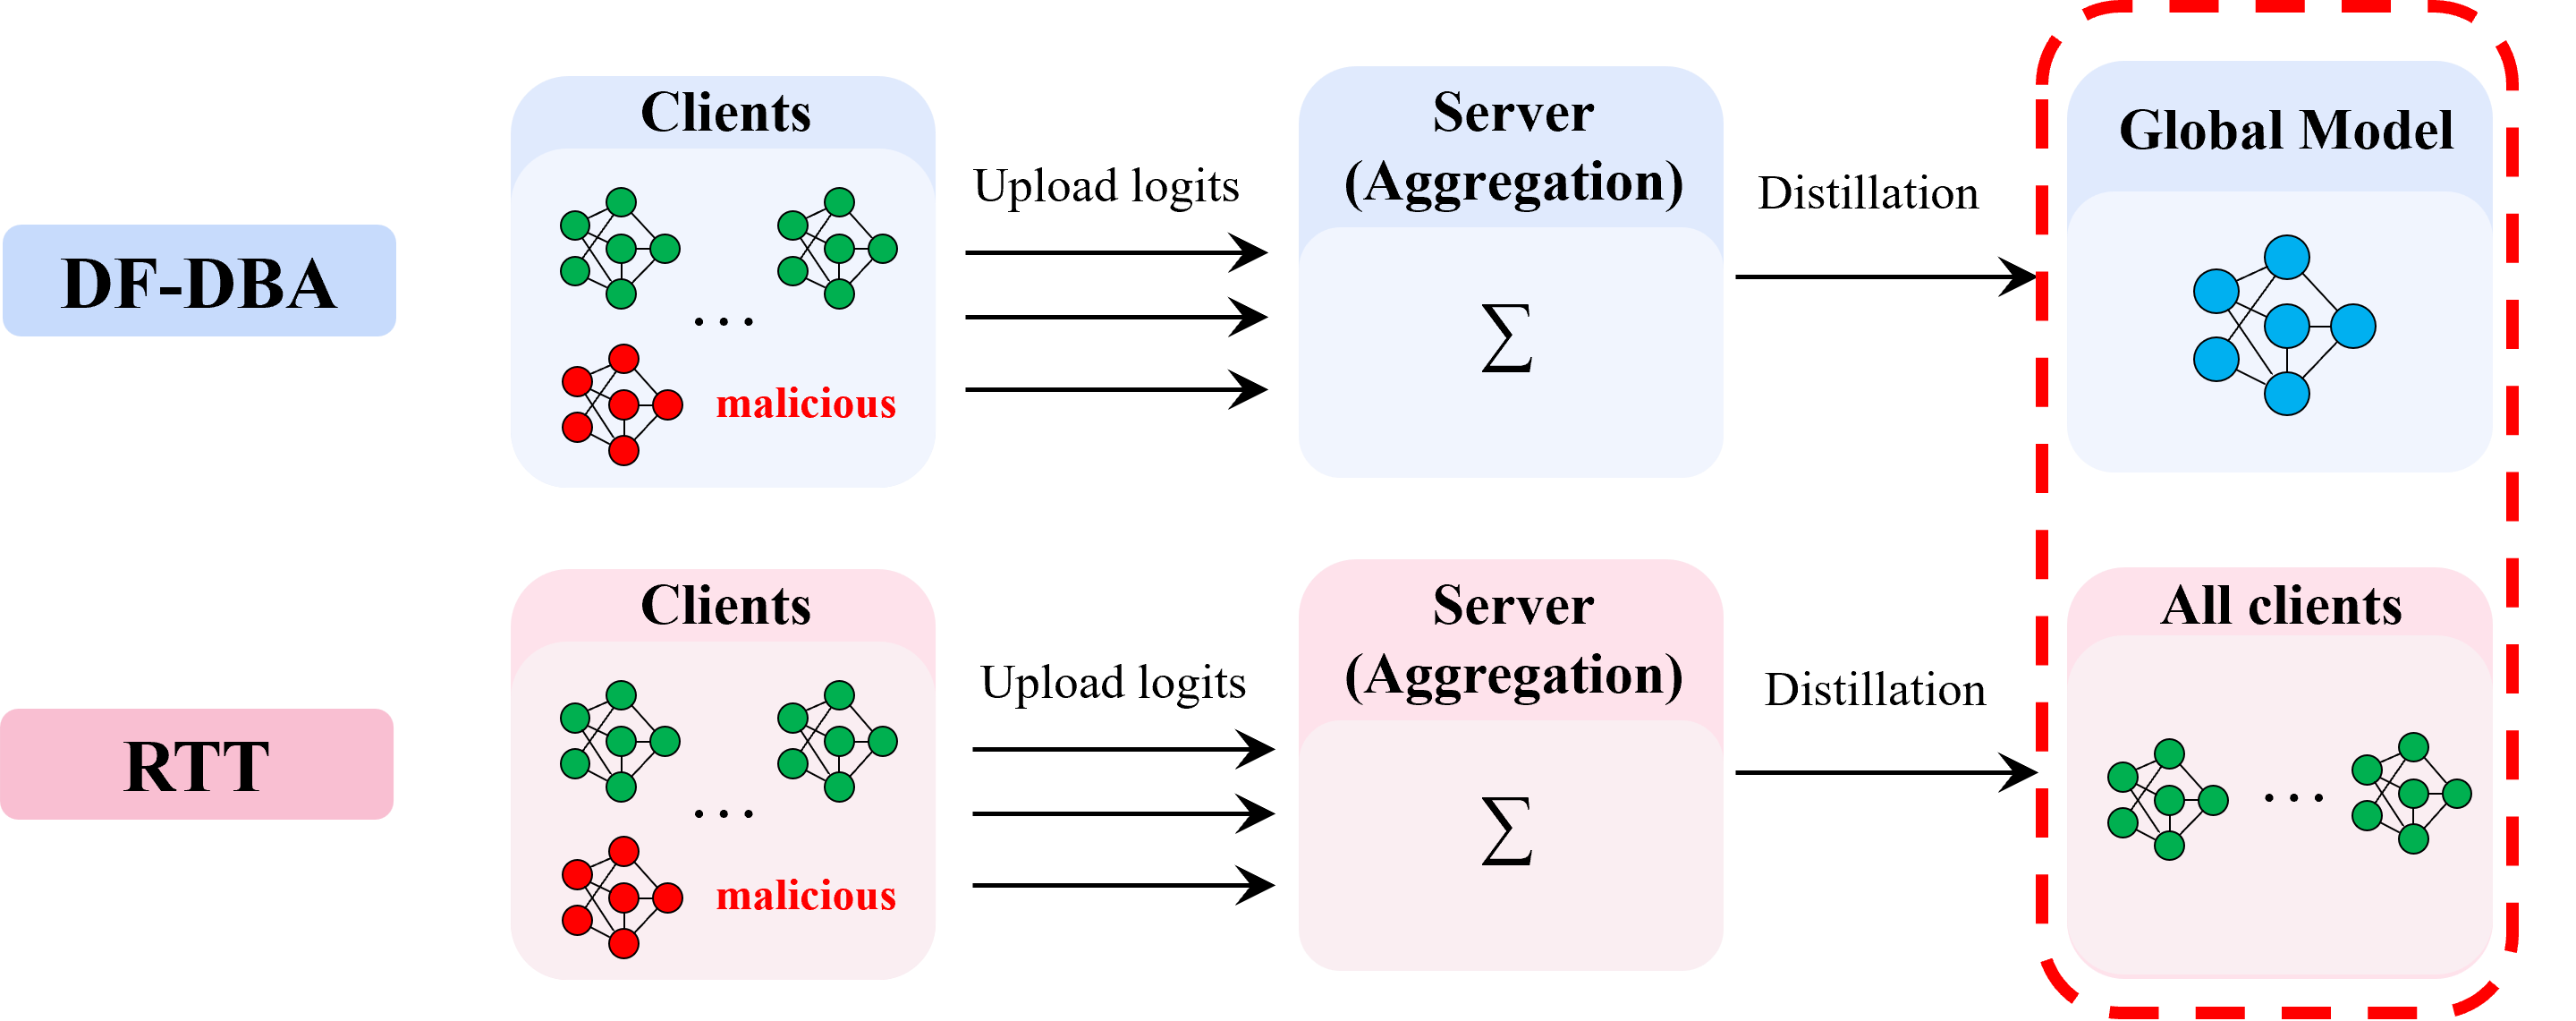
\includegraphics[width=0.8\textwidth]{FDDBA_RTT_Distillation_Comparison.png}
\caption{Comparison of the knowledge distillation frameworks of FD-DBA and RTT.}
\label{fig:fddba_rtt_comparison}
\end{figure}

Based on this relationship, to ensure a fair comparison, we only change FD-DBA's attack targets from the server-maintained global model to multiple heterogeneous client models, while preserving its original attack design and all other training and knowledge propagation procedures.
We then evaluate ASR and ACC on the same client models.

Under the unified evaluation setting, FD-DBA achieves a certain degree of backdoor effectiveness. 
However, the discrepancy between substitute-model distillation and the actual knowledge distillation process, together with the indirect propagation of backdoor associations, weakens its propagation effectiveness. 
In contrast, RTT directly reconstructs trigger--target associations during actual knowledge distillation, achieving higher ASR.

\textbf{(3) Abnormal accuracy results on DBpedia.}

We sincerely thank you for pointing out the abnormal ACC differences among the no-attack setting, Edge-case, and FD-DBA on DBpedia. 
After carefully examining the experimental records, we confirmed that these errors resulted from an oversight during the recording of experimental results, which led to incorrect ACC values for Edge-case and FD-DBA. 
We sincerely apologize for these errors.

We have corrected the corresponding values and updated \textbf{Table IV} in the \textbf{Experimental Results (Baselines)} section of the revised manuscript. 
Furthermore, we have thoroughly checked the other experimental results and confirmed that no similar errors remain. 
We sincerely appreciate your careful review and valuable reminder.

\textbf{(4) Baseline adaptation, attack objectives, evaluation protocols, and hyperparameter tuning.}

We have further clarified the adaptation procedures, attack objectives, evaluation protocols, and hyperparameter tuning settings of the baseline methods under KD-FL in the \textbf{Experimental Setup (Baselines)} section of the revised manuscript.

For SADBA, Edge-case, and Bad-PFL, we retain their original trigger designs and local backdoor training procedures, replacing parameter uploads with logits uploads under the KD-FL protocol, and evaluate ASR using their respective triggers. 
For ManipulatingKD and FDLA, we preserve their original logits manipulation strategies, evaluate ASR using RTT's natural trigger conditions, and assess their original untargeted poisoning effectiveness through ACC. 
FD-DBA is adapted as described in Point (2), retaining its original attack design while unifying the distillation targets and evaluation models.

Regarding the comparability of attack objectives and evaluation protocols, we assign different roles to ASR and ACC according to the attack objectives of each method.
For SADBA, Edge-case, Bad-PFL, FD-DBA, and RTT, ASR is used to evaluate backdoor attack effectiveness, while ACC measures normal classification performance, as preserving normal classification performance is also an important requirement of backdoor attacks.
For ManipulatingKD and FDLA, ACC is used to evaluate their original untargeted poisoning effectiveness and compare the impact of different logits manipulation strategies on ACC.
ASR serves as a supplementary metric to examine whether they can establish targeted backdoor associations, rather than to evaluate the achievement of their original attack objectives.

To ensure the comparability of experimental results, all methods use the same non-IID data settings, malicious client ratio, logits aggregation, and knowledge distillation settings, with ASR and ACC evaluated on the same client models.

For hyperparameter tuning, each baseline retains the trigger structures, attack loss functions, and logits manipulation strategies specified in its original paper. 
Attack-specific parameters, such as poisoning ratios, trigger strengths, and optimization constraints, are further tuned under consistent KD-FL training settings.

\textbf{(5) Attack performance of benign and malicious clients.}

Thank you for this suggestion. 
In Fig.~3 of the original manuscript, we reported the ASR and ACC of RTT across all clients on eight datasets using means and standard deviations. 
The solid lines represent the mean values across all clients, while the shaded regions indicate the standard deviations. 
These results provide an overall view of RTT's attack effectiveness across heterogeneous clients. 
However, we also recognize that this presentation is insufficient to distinguish the attack performance of benign and malicious clients or to show the results for individual model architectures.

Therefore, we have added a client-level analysis on CIFAR-10 in the \textbf{Experimental Results (Client-Level Attack Performance)} section of the revised manuscript. 
Specifically, we report the ASR and ACC of all 20 clients, including 18 benign clients and 2 malicious clients. 
Different markers are used to distinguish benign and malicious clients, and the results are grouped by five model architectures: ResNet-18, AlexNet, VGG-11, DenseNet-121, and CNN-3.

The results show that both benign and malicious clients achieve high ASR, demonstrating that trigger--target associations can be effectively propagated to benign clients with different model architectures through logits aggregation and knowledge distillation. 
The variations in ASR and ACC across clients are mainly attributed to differences in model architectures and local data distributions.
}

\revisedtext{Section II-B, Page [X], Lines [XX--XX]}{[Insert the exact new KD-FL backdoor related-work paragraph here, including the relevant citations.]}



\reviewcomment{ The stealthiness and practical effectiveness of RTT are insufficiently characterized.
RTT avoids modifying the server-maintained distillation dataset and introduces regularization to limit malicious logit deviations. However, these properties alone do not establish that the attack is difficult to detect. Table V reports ASR under several defense methods but does not provide corresponding clean accuracy, detection statistics, or measurements of malicious logit deviations. These results would help support the claimed robustness against defenses. Furthermore, Fig. 5 shows visibly modified explicit-trigger samples. The authors should specify how the random response direction is converted into an input-space trigger, including its magnitude, normalization, and injection procedure. Quantitative measures of trigger visibility and additional evaluation under constrained trigger magnitudes would improve the practical assessment.
}

\authorresponse{We sincerely thank the reviewer for the careful reading of our manuscript and the constructive comments. Your suggestions have helped us further improve the experimental evaluation and result analysis, making the assessment of RTT's performance under defense scenarios and the visibility of explicit triggers more comprehensive and thorough, thereby enhancing the persuasiveness of the experimental results and the credibility of our conclusions. In response to these suggestions, we have expanded the defense experiments and supplemented the explicit-trigger construction procedure, quantitative visibility metrics, and experimental results under different injection magnitudes.

\textbf{First, regarding attack effectiveness and detection statistics under defense mechanisms.}
We have further extended the experimental evaluation under four defense methods. Specifically, RLA and ExpGuard assign lower aggregation weights to suspected clients. Therefore, we adopt the ratio of the average aggregation weight assigned to malicious clients to that assigned to benign clients ($R_w$) to evaluate their defense effectiveness. FedTGD resists attacks by filtering anomalous clients. Accordingly, we use the true positive rate (TPR) of malicious client detection to measure its detection capability. Selective-FD performs defense by filtering unreliable distillation samples on the server side. Therefore, we adopt the natural-trigger sample filtering rate (TFR) to evaluate its defense effectiveness. In addition, we report classification accuracy (ACC) and the average Euclidean distance ($\Delta_z$) between the logits uploaded by malicious clients before and after modification, which measure normal classification performance and the extent of malicious logit modifications, respectively.

The experimental results demonstrate that RTT maintains high ASR and stable ACC under all four defense methods. The $R_w$ values of RLA and ExpGuard are close to 1, indicating that malicious clients are not significantly downweighted. FedTGD achieves a low TPR, indicating that only a small proportion of malicious clients are detected. Similarly, Selective-FD exhibits a low TFR, indicating that most natural-trigger samples are not filtered and can still participate in knowledge distillation.

These results demonstrate that RTT maintains effective backdoor propagation under these defense mechanisms and exhibits a certain degree of defense evasion capability.

\textbf{Second, regarding explicit-trigger construction, visibility, and injection magnitude.}

RTT establishes the association between triggers and the target class using natural-trigger samples without modifying the original data. In the preceding experiments, we have evaluated RTT's core attack mechanism and its attack effectiveness using natural-trigger samples. We recognize that the explicit triggers shown in the previous version of the manuscript may have caused some misunderstanding. These triggers are manually constructed and injected into images for supplementary experiments, which is also a common trigger design practice in existing federated learning backdoor attacks [1, 2, 3]. Therefore, to further investigate the attack effectiveness of RTT under explicit-trigger injection, we supplement our evaluation with conventional explicit-trigger injection experiments.

Specifically, we directly use the random response direction from RTT's natural trigger construction stage as the explicit trigger. First, we apply L2 normalization to the random direction $\mathbf K$ and then scale it by the injection magnitude $\epsilon$. Subsequently, the resulting vector is reshaped to match the predefined local response region and added to the corresponding location of each test image. We have supplemented this procedure in the \textit{Evaluation Metrics} section of the revised manuscript and updated the explicit-trigger ASR definition based on $\hat{y}(\mathbf{x}+\epsilon\hat{\mathbf K})$.

To further evaluate explicit-trigger visibility and attack effectiveness under different injection magnitudes, we extend the original experiments by considering three injection magnitudes, $\epsilon\in\{0,0.5,1.0\}$, where $0$ indicates no trigger injection, $0.5$ represents half of the original injection magnitude, and $1.0$ corresponds to the original injection magnitude. We also introduce the Structural Similarity Index Measure (SSIM) as a quantitative measure of trigger visibility and report ASR, ACC, and SSIM under different injection magnitudes.

The experimental results demonstrate that ASR is close to zero without explicit trigger injection. When $\epsilon=1.0$, RTT achieves high ASR across all datasets. Even when the injection magnitude is reduced to $0.5$, RTT maintains high attack success rates with reduced trigger visibility. Meanwhile, ACC remains stable across different injection magnitudes. These results demonstrate that RTT remains effective under conventional explicit-trigger injection settings and maintains strong attack effectiveness even when the injection magnitude is reduced.

\noindent [1] Q. Yang, P. Yan, X. Wu, J. Zhang, T. Song, Y. Hua, H. Wang, L. Wang, and H. Guan, "Stealthy Backdoor Attack in Federated Learning via Adaptive Layer-wise Gradient Alignment," in \textit{Proceedings of the IEEE/CVF International Conference on Computer Vision (ICCV)}, pp. 29163--29172, 2025.

\noindent [2] C. Xie, K. Huang, P.-Y. Chen, and B. Li, "DBA: Distributed Backdoor Attacks against Federated Learning," in \textit{International Conference on Learning Representations (ICLR)}, 2020.

\noindent [3] T. Liu, Y. Zhang, Z. Feng, Z. Yang, C. Xu, D. Man, and W. Yang, "Beyond Traditional Threats: A Persistent Backdoor Attack on Federated Learning," in \textit{Proceedings of the AAAI Conference on Artificial Intelligence}, vol. 38, no. 19, pp. 21359--21367, 2024.
}
\revisedtext{Section II-B, Page [X], Lines [XX--XX]}{[Insert the exact new KD-FL backdoor related-work paragraph here, including the relevant citations.]}
\end{document}
